\documentclass{proc}

\usepackage{hyperref}
\usepackage{graphicx}

% Header and footer.

\title{\textbf{\tt Music Generation Through LSTM}\\ \textbf{\tt CS 351 - Artificial Intelligence}}
\author{\textbf{\tt Emad Bin Abid, Saman Gaziani}\\ 
\textbf{\tt Habib University, Karachi} \\ {\tt ea02893@st.habib.edu.pk, sg02494@st.habib.edu.pk}\\ \\ {\tt \textbf{Project Report}}}
%\date{{\tt \textbf{Project Report}}}

\begin{document}
\maketitle

\section*{Abstract:}
In this report, we explain the procedure and methodology used to build an automatic music generation system using Long Short Term Memory (LSTM). LSTM is one of the variations of recurrent neural networks and are widely used in sequence-based models. Our project aims to use LSTM units to generate new music compositions after training the model on existing music files. \\ \\
\textbf{Keywords:} Music generation, LSTM, sequence-based models. 

\section*{Introduction:}
Music generation is a time dependent form of art just like speech and video. Therefore, in order to generate music, we had to use sequence-based models. Recurrent neural networks have the tendency to handle sequential data and hence we opted RNNs for our modeling. Vanilla RNNs suffer with two major issues namely \textit{vanishing gradient} and \textit{exploding gradient}. In order to resolve these major issues Long Short Term Memory (LSTM) and Gated Recurrent Units (GRU) are used. Among these two resolutions, we chose LSTM for our project. LSTMs require more number of parameters to be learned but most of the times they give better results as compared to GRUs. The project was mainly divided into two phases. The first phase was primarily related to \textbf{data preprocessing} and the second phase revolved around \textbf{model building}. The tools and technologies used for both phases will be discussed later in detail. We did not face much hurdles in the data collection stage of the first phase. The music files were easily available. The processing stage took a detailed time as we had to explore new tools and libraries for the data preprocessing. The second phase, \textit{model building}, also took a reasonable amount of time as we had to experiment different models and finally come up with a model that could better fit our data. 

\section*{Data Collection:}
We collected our data as audio music files in \textit{midi} format. The genre of data collected was \textit{Jazz}. In order to process data, we used MIT's \textit{music21} library. The library made it easier to extract notes from a MIDI music file. The notes were filtered according to the requirements. After extracting the note names, the notes were saved in a file for later usage. The sequence of notes in music file was arranged and split in a way that it could be fed into the model for training. 

\section*{Model Architecture:}
We tried different model architectures with different number of learning parameters and compared their results. We finally opted the model configuration which best suited our data. The configuration contained two LSTM layers followed by a fully connected dense layer with \textit{softmax} activation. The block diagram of model architecture is given below.
\begin{center}
	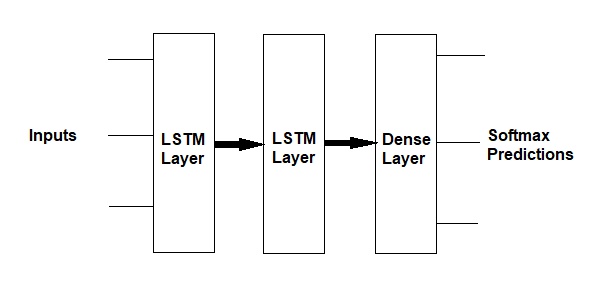
\includegraphics[scale=0.50]{./assets/model-architecture}
\end{center}

\section*{Results and Discussion:}
We tried our final model with different hyper parameters. The hyper parameters include learning rate and number of epochs. Initially, we trained our model with 5 epochs. The model results were very bad. The loss value obtained was 4.8656. The performance of the model is visually shown below. \\ \\
\begin{center}
	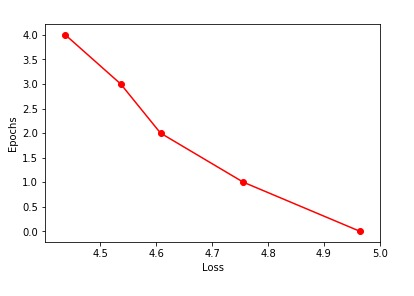
\includegraphics[scale=0.50]{./assets/train-1}
\end{center}

Later, we tried our model on 50 epochs and we observed that the loss was reduced up till 0.0695. The model started producing some really nice piano tunes. The model performance can be visualized as follows. \\ \\
\begin{center}
	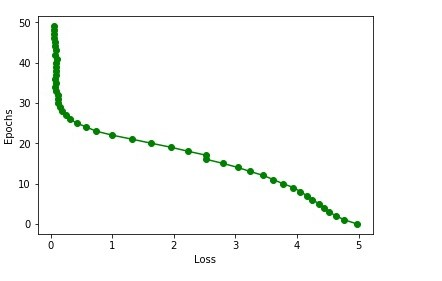
\includegraphics[scale=0.70]{./assets/train-2}
\end{center}


\section*{Tools and Libraries:}
Throughout the project, we used \textbf{Python} as our programming language. Furthermore, following main libraries of Python were used to facilitate our 
project programming.\\ \\
\textbf{For Data Preprocessing:}
\begin{description}
	\item[.] music21
	\item[.] pandas
\end{description}
\textbf{For Model Building:}
\begin{description}
	\item[.] keras
\end{description}

\section*{Future Work:}
The proceedings on the project have not been stopped yet. We plan to continue this project by adding more musical instruments modules such as \textit{Piano}, \textit{Guitar}, \textit{Drums}, \textit{Violin}, etc. Furthermore, we plan to conduct a proper research on measuring and quantifying music similarity.

\section*{Conclusion:}
Our project on music generation through LSTMs takes in MIDI files as input, extracts notes from the music files, coverts them in a textual representation and then after some training process generates new music tunes given that some initial seed notes are provided to it. The model produced some really effective and smooth tunes after running on 50 epochs. The last loss value recorded was 0.0436. 

\end{document}